\section{Theory}
\label{sec:theorie}

Before explaining how exactly a diode laser works, some basics of semiconductors are discussed.

\subsection{Semiconductors}

When looking at the lattice structure of a solid state, the band structure allows for categorisation into three different categories.
In the lattice, the electrons occupy different energy levels. These electrons however do not necessarily occupy the same energy levels, so that,
when looking at the bigger picture, there exists a band structure of electrons.
Here, the valence and conduction bands are most important.
The valence band describes the highest fully occupied band at $T = \SI{0}{\kelvin}$ and it separated from the (almost always higher energy) conduction band
by a band gap.
The conduction band on the other hand is not fully occupied and therefore allows for free electron movement inside the band, meaning in turn that its electrons
can contribute to the solid's electrical conductivity.\\

Depending on the size of this band gap, solids are classified into insulators, semiconductors and metals.
While for insulators, the band gap is so large that even when thermally stimulated, it cannot be bridged.
Metals, on the other hand, have a negative band gap; even at low temperatures, they show high conductivity.
Semiconductors lie in between; their band gap is smaller than that of insulators, but not zero.
This means that at low temperatures, they act similarly to an insulator, but at higher temperatures become more conductive.

\subsubsection{Doping}

To change the conductive properties of a semiconductor, it is often helpful to use a process called Doping.
It describes the introduction of foreign atoms into the lattice.
Depending on whether the dopants possess more or less electrons than the lattice atoms, they are called donors or acceptors respectively.
Doping with donors is called n-doping and doping with acceptors is called p-doping.
Introducing the dopants into the lattice changes the band structure of the semiconductor and thereby its conductivity. \\

\subsubsection{The p-n Junction}
Here, a combination of p- and n-doping is used.
In this so called p-n junction, as seen in \autoref{fig:p-n_junction}, electrons can move into the valence band of the p-doped material
by recombining with its holes, leading to a charge density where this recombination happens.
The charge density creates a potential that can be overcome by applying a voltage, so that the electrons can now fill the conduction band.
Thus a phenomenon called population inversion is created, where electrons occupy higher energy states more than the ground state.

\begin{figure}[H]
    \centering
    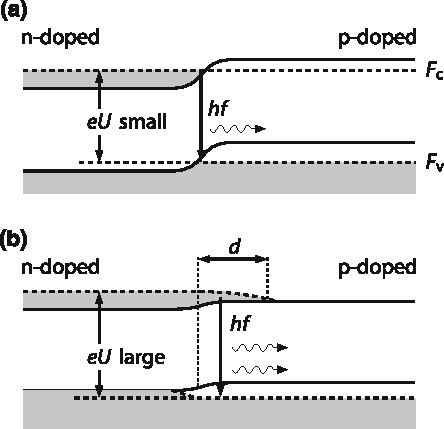
\includegraphics{figures/p-n_junction.pdf}
    \caption{Visualisation of the band structure and the effect of applying a voltage to the p-n junction \cite{laser}.}
    \label{fig:p-n_junction}
\end{figure}


\subsection{Diode Lasers}
Inside a diode laser, there is a layered chip of a n-doped and p-doped semiconductor separated by the aforementioned p-n junction as seen in \autoref{fig:diode}.

\begin{figure}[H]
    \centering
    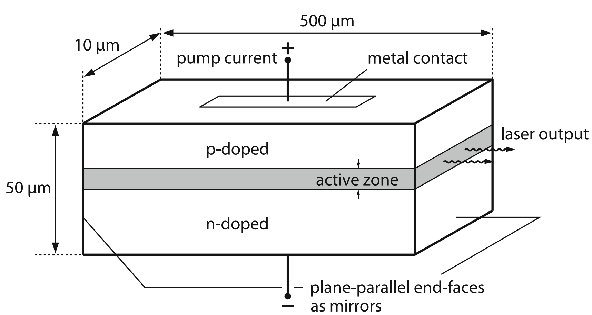
\includegraphics{figures/diode_laser_chip.pdf}
    \caption{Schematic representation of a diode laser chip \cite{laser}.}
    \label{fig:p-n_junction}
\end{figure}

If a low voltage is applied, the electrons are excited into higher energy states, emitting photons as they return to their lower energy states.
Depending on the energy gap between excited and unexcited state, the photons wavelength differs.
In this low voltage environment, the chip acts as a LED (Light Emitting Diode). \\
If the voltage is high enough and population inversion is achieved, the light emitted by the electrons is amplified via stimulated emission,
as seen in \autoref{fig:emission}.

\begin{figure}[H]
    \centering
    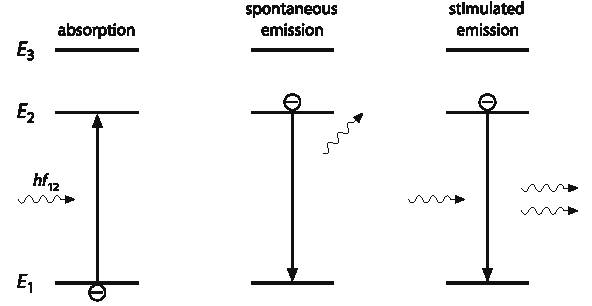
\includegraphics{figures/emission.pdf}
    \caption{Absorption, spontaneous and stimulated emission \cite{laser}.}
    \label{fig:emission}
\end{figure}


\subsubsection{Inner Cavity}
One end of the diode is fully and the other one partially reflective, creating an inner cavity that further amplifies resonating photon modes
and thus creating standing waves inside the cavity.
In this configuration, the diodes lases only selected modes of a still broad spectrum, emerging as a highly diverging elliptical beam.


\subsubsection{Outer Cavity}
To restrict the broad spectrum, an outer cavity is installed.
As shown in \autoref{fig:outercavity}, one possibility is to employ a grating, here specifically in Littrow configuration.
The lense in front of the grating aligns the beam so that it no longer diverges.
The grating is rotated so that it reflects the first order is reflected back into the chip and the zeroth order maximum is used as the primary beam.
Together with the highly reflective coating on the backside of the chip, it forms an outer cavity with its own modes.

\begin{figure}[H]
    \centering
    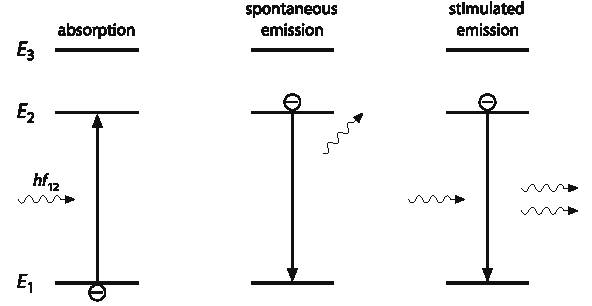
\includegraphics{figures/emission.pdf}
    \caption{Absorption, spontaneous and stimulated emission \cite{teachspin}.}
    \label{fig:emission}
\end{figure}

\subsubsection{Mode Hopping}

The laser produces the mode with the highest gain.

\begin{figure}[H]
    \centering
    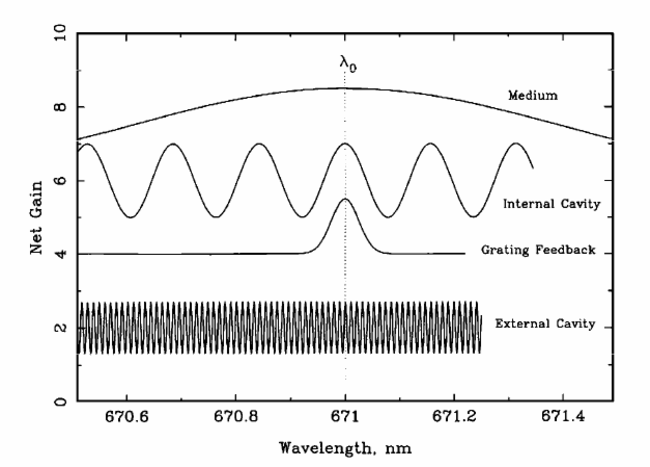
\includegraphics{figures/gain.pdf}
    \caption{Different components of the diode laser and their contributions to the highest gain mode \cite{teachspin}.}
    \label{fig:gain}
\end{figure}

As visualised in \autoref{fig:gain}, the highest gain mode is determined from the highest gain modes from both cavities in addition
to the mode amplified by the grating.
If now for example the outer cavity is adjusted by turning the grating or the diode is heated, so too shift the modes they amplify.
At some point, the maximum of the sum of the two feedbacks changes frequency, as seen in \autoref{fig:modehopping},
producing a new highest gain mode.
This phenomenon is called mode hopping.

\begin{figure}[H]
    \centering
    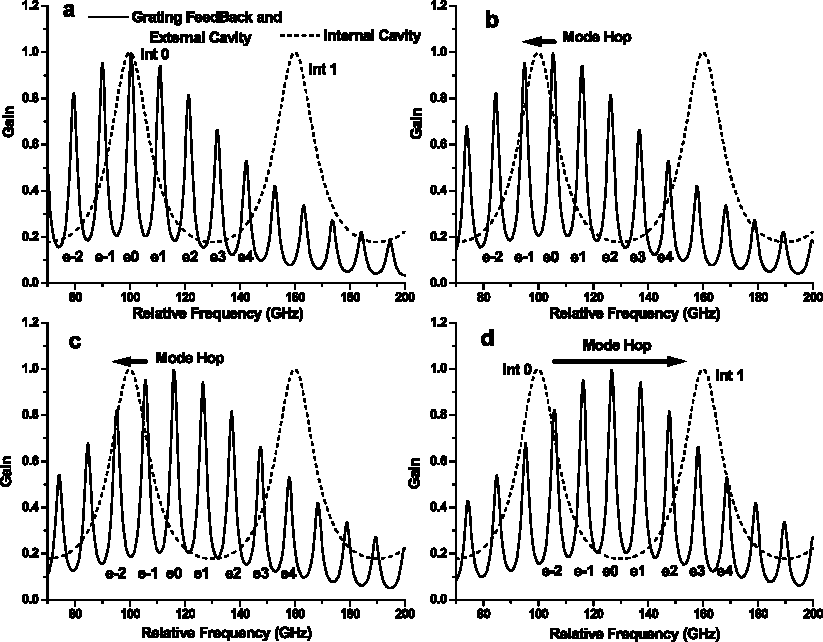
\includegraphics{figures/modehopping.pdf}
    \caption{Representation of how changing cavity lengths affects feedback and mode hopping \cite{teachspin}.}
    \label{fig:modehopping}
\end{figure}


\subsection{Absorption Spectroscopy}

Absorption spectroscopy allows for structural analysis by observing the absorption spectrum of a material.
Certain wavelengths of light are absorbed by the substance, exciting its atoms.
When these excited atoms relax, they release photons.
As they are not released in the direction of the laser, a decrease in beam intensity can be observed.
\autoref{fig:rubidium} shows energy states and absorption spectrum for Rubidium.

\begin{figure}[H]
    \centering
    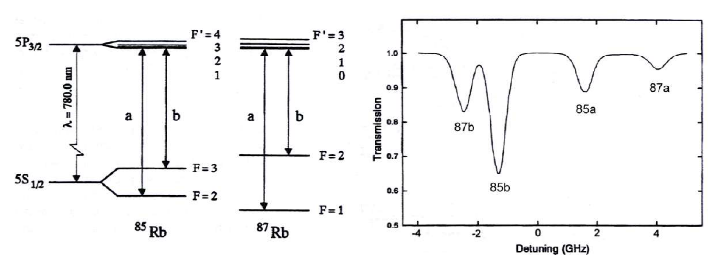
\includegraphics{figures/absorption_spectroscopy.pdf}
    \caption{Energy states and absorption spectrum of Rubidium, showing the different minima for different Rubidium isotopes and excitations \cite{teachspin}.}
    \label{fig:rubidium}
\end{figure}


